\documentclass[11pt]{article}

\usepackage{nmrdoc}
\usepackage{siunitx}
\usepackage{bm}
\usepackage{tikz}
\usetikzlibrary{positioning}

\sisetup{per-mode=symbol}
\DeclareSIUnit{\angstrom}{\text{\AA}}
\DeclareSIUnit{\ppm}{ppm}
\DeclareSIUnit{\elementarycharge}{e}

\newcommand{\code}[1]{\texttt{#1}}
\newcommand{\dd}{\,d}
\newcommand{\stf}{\operatorname{STF}}

\setlength{\parindent}{0pt}
\setlength{\parskip}{0.48em}
\emergencystretch=4em
\AtBeginDocument{\raggedright}

\begin{document}
\NmrTitle{The Physics Architecture Between the Shielding Calculators}
\tableofcontents
\clearpage

\section{The Object Being Shadowed}

All twelve calculators point at the same physical object, even when they do not
compute it. That object is the nuclear magnetic shielding tensor. Place a
nucleus in an externally applied magnetic field \(\bm B_0\). The electrons move
and polarize in response. Their induced motion creates a secondary magnetic
field at the nucleus, so the nucleus sees
\[
  \bm B_{\mathrm{nuc}}=(\bm I-\bm\sigma)\bm B_0 .
\]
\(\bm B_{\mathrm{nuc}}\) is the magnetic field at the nucleus. \(\bm I\) is
the \(3\times3\) identity matrix. \(\bm\sigma\) is the shielding tensor: a
dimensionless \(3\times3\) linear-response coefficient. Its entry
\(\sigma_{ab}\) says how an applied-field component along direction \(b\)
reduces or redirects the magnetic field component along direction \(a\) at the
nucleus. The minus sign is the shielding convention: positive shielding means
the induced electronic field screens the applied field.

This definition is already a map. A molecule is not a sphere. If the applied
field is turned relative to a peptide plane, an aromatic ring, a hydrogen bond,
or a water dipole, the induced electronic current need not point in the same
direction as before. A scalar chemical shift is the shadow cast by this tensor
after orientational averaging, reference subtraction, and a sign convention. The
calculators keep the tensorial shadow before that collapse whenever the code has
a rank-2 geometric object to emit.

Ramsey's quantum theory gives the source of the tensor: shielding is a
second-order response of the electronic state to a nuclear magnetic moment and
an external magnetic field \cite{ramsey1950,facelli2011}. In the current-density
picture, the same response can be written as a Biot--Savart field generated by
the current induced by \(\bm B_0\):
\[
  \sigma_{ab}(I)
  =
  -\frac{\mu_0}{4\pi}
  \int
  \frac{
    \left[
      \left(\partial \bm j(\bm x)/\partial B_{0,b}\right)
      \times
      (\bm R_I-\bm x)
    \right]_a
  }
  {|\bm R_I-\bm x|^3}
  \dd^3 x .
\]
\(\bm R_I\) is the position of nucleus \(I\). \(\bm x\) is an electronic
position in space. \(\bm j(\bm x)\) is the electronic current density. The
derivative \(\partial \bm j/\partial B_{0,b}\) is the part of that current
which changes linearly when the applied field component \(B_{0,b}\) is changed.
The cross product and inverse-cube denominator are the Biot--Savart kernel:
they turn current at \(\bm x\) into magnetic field at the nucleus. The leading
minus sign converts induced field into shielding by the convention above.

None of the geometric calculators evaluates this integral over the true quantum
current density. They replace pieces of the electronic response by classical
sources: a current loop, a susceptibility axis, a point charge, a multipole, a
hydrogen-bond geometry, a dispersion contact, or a solvent shell. The output is
therefore a geometric kernel until a calibration step attaches the missing
response coefficient. LarsenHBond is the partial exception: its tables already
contain DFT shielding-difference tensors in \(\si{\ppm}\), but those tensors
are still local empirical terms, not a complete chemical shift.

\section{The Shared Tensor Language}

The code stores a \(3\times3\) tensor \(\bm X\) by splitting its nine Cartesian
entries into three pieces. This is not a diagonalization and not a choice of
principal axes. It is a closed-form change of coordinates on the tensor entries.

The first piece is the scalar trace average,
\[
  T_0=\frac{1}{3}\operatorname{tr}\bm X
  =\frac{X_{xx}+X_{yy}+X_{zz}}{3}.
\]
It is the part proportional to the identity matrix. For a true shielding tensor,
this is the isotropic shielding.

The second piece is the antisymmetric part, stored as a three-component vector,
\[
  \bm T_1 =
  \frac12
  \begin{pmatrix}
    X_{yz}-X_{zy}\\
    X_{zx}-X_{xz}\\
    X_{xy}-X_{yx}
  \end{pmatrix}.
\]
It records the transpose-odd part of the tensor. Standard isotropic solution
NMR usually does not observe this part directly, but several code kernels are
asymmetric, so the representation keeps it.

The third piece is the symmetric traceless matrix
\[
  \bm S=\frac{\bm X+\bm X^{\mathsf T}}{2}-T_0\bm I,
  \qquad
  \operatorname{tr}\bm S=0 .
\]
Symmetric means \(S_{ab}=S_{ba}\). Traceless means the three diagonal entries
sum to zero. Those two conditions leave five independent numbers. The code packs
them as
\[
  \bm T_2 =
  \begin{pmatrix}
    \sqrt2\,S_{xy}\\
    \sqrt2\,S_{yz}\\
    \sqrt{3/2}\,S_{zz}\\
    \sqrt2\,S_{xz}\\
    (S_{xx}-S_{yy})/\sqrt2
  \end{pmatrix}.
\]
The \(\sqrt2\) factors on the off-diagonal entries pay for double counting:
\(S_{xy}\) appears twice in the full symmetric matrix, as \(S_{xy}\) and
\(S_{yx}\). The diagonal factors do the same accounting for the two remaining
diagonal degrees of freedom after the trace is removed. With these constants,
\(\sum_m T_{2m}^2=\sum_{ab}S_{ab}^2\). The five stored values have the same
length as the underlying symmetric traceless matrix measured by the Frobenius
norm.

In plain representation terms: the nine components of a \(3\times3\) tensor
split as \(1+3+5\). One number is the trace average. Three numbers are the
antisymmetric twist. Five numbers are the pure orientation-dependent stretch
and squeeze. The file order used throughout the calculators is
\[
  [T_0,T_{1x},T_{1y},T_{1z},
    T_{2,-2},T_{2,-1},T_{2,0},T_{2,+1},T_{2,+2}] .
\]

\section{The Kernel That Keeps Returning}

The classical kernel at the centre of the architecture is the second derivative
of \(1/\rho\). Let \(\bm\rho=\bm r-\bm s\) be the vector from a source point
\(\bm s\) to an observation point \(\bm r\), let
\(\rho=|\bm\rho|\), and let \(\delta_{ab}\) be one when Cartesian indices
\(a\) and \(b\) are equal and zero otherwise. Then
\[
  D_{ab}(\bm\rho)
  =
  \frac{\partial^2}{\partial \rho_a\partial \rho_b}
  \frac{1}{\rho}
  =
  \frac{3\rho_a\rho_b-\delta_{ab}\rho^2}{\rho^5}
  =
  \frac{3\hat\rho_a\hat\rho_b-\delta_{ab}}{\rho^3},
\]
where \(\hat{\bm\rho}=\bm\rho/\rho\). This matrix is symmetric and traceless.
Along the line of sight it has eigenvalue \(+2/\rho^3\). In the two transverse
directions it has eigenvalue \(-1/\rho^3\). The three eigenvalues sum to zero.

This same object appears with different physical names. In magnetostatics, it
is the field shape of a point magnetic dipole:
\[
  B_a(\bm r)\propto D_{ab}(\bm\rho)m_b ,
\]
where \(m_b\) is component \(b\) of the dipole moment. In electrostatics, it is
the Hessian of a point-charge potential, and therefore the electric-field
gradient away from the charge. In both cases, the shape is the same because
both fields descend from \(1/\rho\).

If a source has a unit axis \(\hat{\bm u}\), the scalar made by looking along
that axis is the double contraction
\[
  f(\bm\rho,\hat{\bm u})
  =
  \hat u_a D_{ab}(\bm\rho)\hat u_b
  =
  \frac{3\cos^2\theta-1}{\rho^3},
  \qquad
  \cos\theta=\hat{\bm\rho}\cdot\hat{\bm u}.
\]
This is the two-lobed dipolar angular law. It is positive near the source axis,
negative broadside, and zero when \(\cos^2\theta=1/3\), the magic angle near
\(\ang{54.7}\). McConnell, RingSusceptibility, and HBond all write this scalar
as the trace average \(T_0\) of their full asymmetric kernel. Dispersion uses
the same angular matrix but replaces the inverse-cube distance law with an
inverse-sixth-power contact law. WaterField and APBSField use the same
second-derivative structure as an electric-field-gradient tensor. Haigh--Mallion
integrates it over a ring surface. PiQuadrupole differentiates it two more
times.

\section{One Network}

\begin{figure}[ht]
\centering
\resizebox{\textwidth}{!}{%
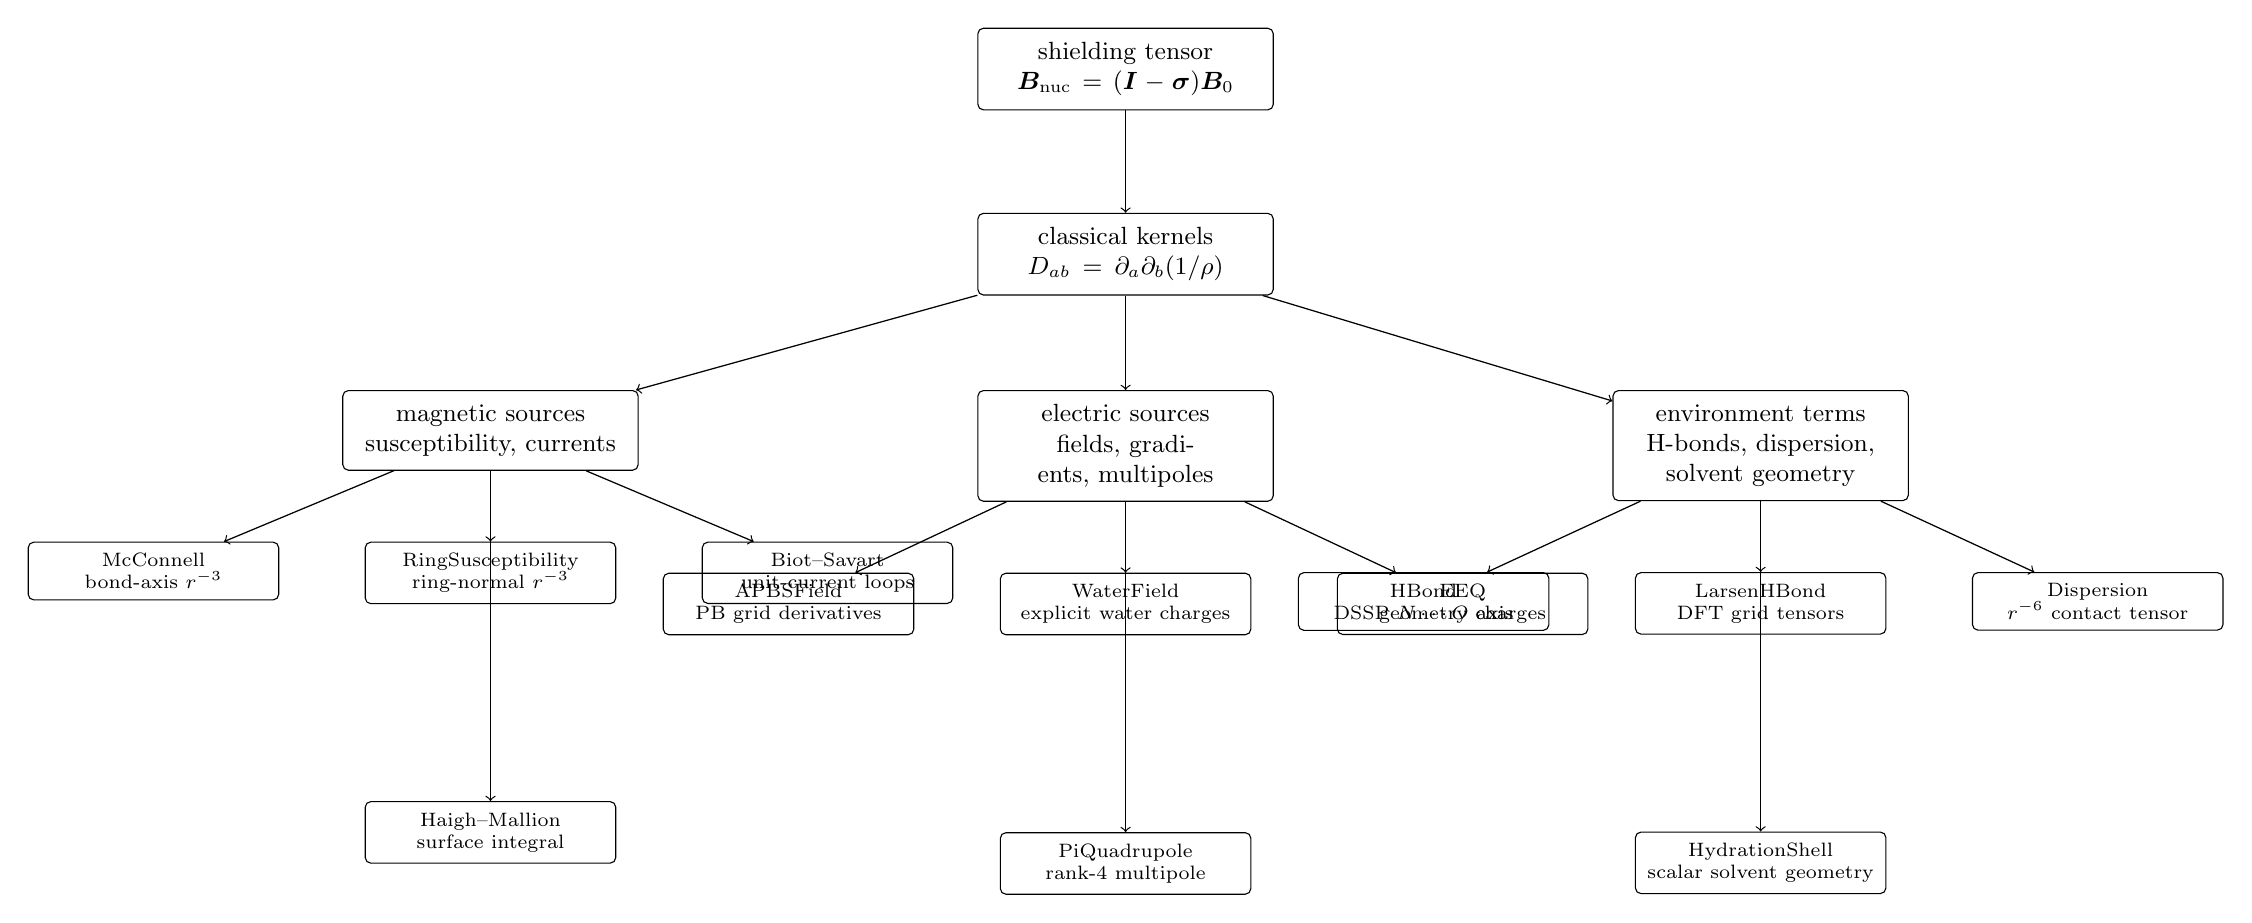
\begin{tikzpicture}[
  node distance=1.3cm and 1.0cm,
  box/.style={draw, rounded corners=2pt, align=center, inner sep=5pt,
              font=\small, text width=3.4cm},
  smallbox/.style={draw, rounded corners=2pt, align=center, inner sep=4pt,
                   font=\scriptsize, text width=2.9cm},
  arrow/.style={->, line width=0.45pt}
]
  \node[box] (shield) {shielding tensor\\\(\bm B_{\mathrm{nuc}}=(\bm I-\bm\sigma)\bm B_0\)};
  \node[box, below=of shield] (kernel) {classical kernels\\\(D_{ab}=\partial_a\partial_b(1/\rho)\)};

  \node[box, below left=1.2cm and 4.3cm of kernel] (mag) {magnetic sources\\susceptibility, currents};
  \node[box, below=1.2cm of kernel] (elec) {electric sources\\fields, gradients, multipoles};
  \node[box, below right=1.2cm and 4.3cm of kernel] (env) {environment terms\\H-bonds, dispersion, solvent geometry};

  \node[smallbox, below left=0.9cm and 0.8cm of mag] (mc) {McConnell\\bond-axis \(r^{-3}\)};
  \node[smallbox, below=0.9cm of mag] (ringchi) {RingSusceptibility\\ring-normal \(r^{-3}\)};
  \node[smallbox, below right=0.9cm and 0.8cm of mag] (bs) {Biot--Savart\\unit-current loops};
  \node[smallbox, below=2.5cm of ringchi] (hm) {Haigh--Mallion\\surface integral};

  \node[smallbox, below left=0.9cm and 0.8cm of elec] (apbs) {APBSField\\PB grid derivatives};
  \node[smallbox, below=0.9cm of elec] (water) {WaterField\\explicit water charges};
  \node[smallbox, below right=0.9cm and 0.8cm of elec] (eeq) {EEQ\\geometry charges};
  \node[smallbox, below=2.5cm of water] (pq) {PiQuadrupole\\rank-4 multipole};

  \node[smallbox, below left=0.9cm and 0.8cm of env] (hb) {HBond\\DSSP \(N\cdots O\) axis};
  \node[smallbox, below=0.9cm of env] (larsen) {LarsenHBond\\DFT grid tensors};
  \node[smallbox, below right=0.9cm and 0.8cm of env] (disp) {Dispersion\\\(r^{-6}\) contact tensor};
  \node[smallbox, below=2.5cm of larsen] (hydr) {HydrationShell\\scalar solvent geometry};

  \draw[arrow] (shield) -- (kernel);
  \draw[arrow] (kernel) -- (mag);
  \draw[arrow] (kernel) -- (elec);
  \draw[arrow] (kernel) -- (env);

  \draw[arrow] (mag) -- (mc);
  \draw[arrow] (mag) -- (ringchi);
  \draw[arrow] (mag) -- (bs);
  \draw[arrow] (mag) -- (hm);
  \draw[arrow] (elec) -- (apbs);
  \draw[arrow] (elec) -- (water);
  \draw[arrow] (elec) -- (eeq);
  \draw[arrow] (elec) -- (pq);
  \draw[arrow] (env) -- (hb);
  \draw[arrow] (env) -- (larsen);
  \draw[arrow] (env) -- (disp);
  \draw[arrow] (env) -- (hydr);
\end{tikzpicture}}
\caption{The calculators are not isolated formulas. They are different
classical reductions of the same response problem: electronic currents create
shielding, and the code measures geometric kernels that could organize those
currents after calibration.}
\end{figure}

The diagram separates source mechanisms, not code ownership. The ring-current
calculators live together because they all ask how an aromatic ring responds to
\(\bm B_0\), but they make different classical replacements for the unknown
quantum current. The electrostatic calculators live together because they all
read the local potential landscape: first derivatives as fields, second
derivatives as field gradients, and higher derivatives as multipoles. The
environment calculators sit on the boundary: they do not all emit tensors, but
they report the solvent, contact, and hydrogen-bond geometry that can change the
electronic response behind \(\bm\sigma\).

\section{Magnetic Susceptibility: Bonds, Rings, and H-Bonds}

A small anisotropic magnetic object has a preferred axis. Call that unit axis
\(\hat{\bm u}\). For a covalent bond, \(\hat{\bm u}\) is the bond direction.
For RingSusceptibility, it is the aromatic ring normal. For HBond, it is the
donor-\(N\) to acceptor-\(O\) direction supplied after DSSP has identified the
backbone hydrogen bond \cite{kabsch1983}. Let \(\bm m\) be the source midpoint
or ring centre, let \(\bm r_i\) be the target atom position, and define
\[
  \bm d=\bm r_i-\bm m,\qquad
  r=|\bm d|,\qquad
  \hat{\bm d}=\bm d/r,\qquad
  c=\hat{\bm d}\cdot\hat{\bm u}.
\]
\(\bm d\) points from the source centre to the target atom. \(r\) is the
centre-to-atom distance. \(c\) is the cosine of the angle between the
observation direction and the source axis.

The shared full tensor used by this family is
\[
  M_{ab}
  =
  \frac{
    9c\,\hat d_a\hat u_b
    -3\hat u_a\hat u_b
    -\left(3\hat d_a\hat d_b-\delta_{ab}\right)}
  {r^3}.
\]
The first term is the dyadic product of the observation direction and the
source axis, weighted by the angle \(c\). It is generally asymmetric, so it can
create \(T_1\). The second term projects onto the source axis. The third term
is the negative of the dipolar kernel \(D_{ab}\). The trace identity is
\[
  \frac{1}{3}\operatorname{tr}\bm M
  =
  \frac{3c^2-1}{r^3}.
\]
Thus the familiar McConnell scalar is not a separate law replacing the tensor;
in this code it is the \(T_0\) component of the full geometric tensor.

McConnell applies this expression to accepted covalent bonds. It collapses each
bond to its midpoint and axis, applies distance and near-field exclusions, and
sums unit-weight tensors in \(\si{\angstrom^{-3}}\). It does not multiply by a
bond susceptibility anisotropy. It therefore preserves the angular source
geometry from McConnell's long-range shielding theory \cite{mcconnell1957}, but
not the material coefficient that would turn the geometry into physical
shielding.

RingSusceptibility makes the substitution
\(\hat{\bm u}\mapsto\hat{\bm n}\), where \(\hat{\bm n}\) is the fitted aromatic
ring normal. It is the point-susceptibility version of an aromatic ring: the
whole ring becomes a small anisotropic magnetic object at its centre. It shares
the same \(r^{-3}\) kernel as McConnell, but the axis is a plane normal rather
than a bond direction. The code does not use ring-current intensities or
Johnson--Bovey lobe offsets in this calculator; every accepted aromatic ring
has unit geometric weight. Case's DFT calibration of aromatic ring-current
effects is the natural ancestor for the later calibration step, not a coefficient
already applied here \cite{case1995}.

HBond makes a different substitution:
\(\hat{\bm u}\mapsto\hat{\bm h}\), the donor-\(N\) to acceptor-\(O\) unit
direction, with the source point at the \(N\cdots O\) midpoint. Its physical
premise is not that the hydrogen bond is a literal magnetic susceptibility
rod. It is that backbone hydrogen bonding reorganizes electronic structure, and
that the \(N\cdots O\) line supplies a strong local axis for the rank-2
shielding response. The code uses the same unit-weight McConnell-family tensor
as a geometric proxy. It does not multiply by DSSP energy, donor--hydrogen
angle, charge, or an empirical shielding coefficient. The broader physical
claim that hydrogen-bond networks strongly affect amide-proton shifts is
supported by quantum and empirical studies of backbone hydrogen bonding
\cite{parker2006,larsen2015}.

The shared origin is the dipolar kernel. The divergence is the identity of the
axis and the source list. McConnell gets axes from covalent bonds.
RingSusceptibility gets axes from aromatic planes. HBond gets axes from a
hydrogen-bond assignment. They are the same symbolic machine with different
source semantics.

\section{Aromatic Ring Currents}

Aromatic rings are special because they offer a more literal current picture.
The applied magnetic field threads the \(\pi\)-electron system. In a classical
model that response is a circulating current, and a current produces magnetic
field by the Biot--Savart law. The canonical ring-current literature begins in
the pre-digital era and is carried through later reviews and calibrations
\cite{pople1956,johnson1958,haigh1979,case1995,boyd2002}. The code implements
three different reductions of that idea.

BiotSavart keeps the current-loop picture. For a current \(I\) flowing along a
curve \(C\), the magnetic field at a point \(\bm r\) is
\[
  \bm B(\bm r)
  =
  \frac{\mu_0 I}{4\pi}
  \oint_C
  \frac{\dd\bm\ell\times(\bm r-\bm s)}
       {|\bm r-\bm s|^3}.
\]
\(\dd\bm\ell\) is a small directed segment of the current path at source point
\(\bm s\). The Johnson--Bovey model replaces an aromatic ring by two displaced
polygonal loops, one on each side of the fitted ring plane. The code evaluates
each straight segment by a closed-form finite-wire expression, sums the two
offset polygons with a unit \(\SI{1}{\nano\ampere}\) current, and then forms
the shielding-like kernel
\[
  G_{ab}=-10^6\,B^{(1)}_a n_b .
\]
\(B^{(1)}_a\) is component \(a\) of the unit-current magnetic field at the
target atom. \(n_b\) is component \(b\) of the ring normal. The outer product
says that only the applied-field component normal to the ring drives this
current in the model, and the resulting secondary field can point in any
Cartesian direction. The matrix has rank at most one and can be asymmetric.
The code records the ring-current intensity for provenance but does not multiply
it into the tensor.

Haigh--Mallion keeps the dipole-field kernel and changes the source from a wire
to a surface. For a target atom at \(\bm r\), a point \(\bm s\) on the ring
surface, and \(\bm\rho=\bm r-\bm s\), the raw surface tensor is
\[
  H_{ab}(\bm r)
  =
  \int_S
  \left(
    \frac{3\rho_a\rho_b}{\rho^5}
    -\frac{\delta_{ab}}{\rho^3}
  \right)
  \dd S .
\]
\(S\) is the fan-triangulated aromatic ring surface and \(\dd S\) is a surface
area element. The integrand is the same \(D_{ab}\) kernel. The code then
contracts this surface response with the ring normal and forms
\[
  V_a=H_{ab}n_b,
  \qquad
  G_{ab}=-V_a n_b .
\]
The raw \(\bm H\) is symmetric and traceless in exact arithmetic because it is
an integral of symmetric traceless kernels. The reported \(\bm G\) is the
rank-at-most-one outer product after the normal contraction. It can have
\(T_0\), \(T_1\), and \(T_2\). Like BiotSavart, the result is an unscaled
geometric kernel.

RingSusceptibility is the point-source limit of the same family. It does not
integrate wires or surfaces. It uses the ring normal in the McConnell-family
closed form from the previous section. That makes it cheaper and more local,
but it carries less information about ring extent and current path.

These three ring calculators therefore disagree in a useful way. BiotSavart
asks what field a pair of current loops would produce. Haigh--Mallion asks what
field a sheet of dipole kernels over the ring interior would produce.
RingSusceptibility asks what an anisotropic point source at the centre would
produce. They share an applied-field projection onto the ring normal and a
secondary magnetic field at the target atom. They diverge in what they believe
the ring current is between those two events.

\section{Electric Fields, Gradients, and Charges}

Electric fields enter shielding because the electron cloud that responds to
\(\bm B_0\) is also shaped by electrostatic environment. Buckingham's classic
expansion writes shielding changes as functions of local electric fields and
electric-field gradients \cite{buckingham1960}. In the code, those response
coefficients are outside the calculators. The calculators report the field or
gradient that such a coefficient could multiply.

For a point charge \(q\) at source point \(\bm s\), a target point \(\bm r\),
and \(\bm\rho=\bm r-\bm s\), the potential is proportional to \(q/\rho\). Its
first derivative gives an electric field up to a sign convention, and its
second derivative gives a rank-2 field-gradient tensor:
\[
  V_{ab}
  =
  k_e q
  \left(
    \frac{3\rho_a\rho_b}{\rho^5}
    -\frac{\delta_{ab}}{\rho^3}
  \right).
\]
\(k_e\) is the Coulomb conversion constant in the code's
\(\si{\volt\angstrom}\) units when charges are in elementary-charge units and
distances are in \(\si{\angstrom}\). Again the bracket is the dipolar kernel.
The tensor is symmetric and traceless away from the charge.

WaterField evaluates this expression directly for explicit solvent waters. A
water molecule enters the sum when its oxygen lies inside the configured oxygen
cutoff; then all three point-charge sites contribute. The vector channel uses
the code's target-to-charge displacement convention, so it is the gradient of
the potential with the sign used by WaterField, not necessarily the textbook
\(-\nabla\phi\) direction. The tensor channel is unaffected by reversing
\(\bm\rho\) because it contains \(\rho_a\rho_b\). After the point-charge sum,
the code removes trace residue and writes the five \(T_2\) components. This is
explicit solvent electrostatics with no continuum reaction field, no Ewald
tail, and no induced polarization inside the calculator.

APBSField obtains the same local objects by a different route. APBS solves a
linearized Poisson--Boltzmann problem for a solvated protein potential on a
grid \cite{baker2001}. The C++ calculator receives only the scalar potential
\(\phi\), not APBS-internal fields. At atom position \(\bm r_i\), with grid
spacing \(h_a\) along Cartesian axis \(a\), it computes
\[
  E_a(\bm r_i)
  =
  -\frac{
    \phi(\bm r_i+h_a\hat{\bm e}_a)
    -
    \phi(\bm r_i-h_a\hat{\bm e}_a)}
  {2h_a},
\]
where \(\hat{\bm e}_a\) is the unit vector along axis \(a\). The minus sign is
the electrostatic convention \(\bm E=-\nabla\phi\). It then computes
\[
  G_{ab}(\bm r_i)
  =
  \frac{
    E_a(\bm r_i+h_b\hat{\bm e}_b)
    -
    E_a(\bm r_i-h_b\hat{\bm e}_b)}
  {2h_b}.
\]
\(G_{ab}\) is the derivative of field component \(a\) with respect to coordinate
\(b\). The code symmetrizes this finite-difference matrix and subtracts its
trace before emitting the \(T_2\) field-gradient feature. Compared with
WaterField, APBSField trades explicit water molecules for dielectric boundary
and ionic screening. Both calculators end at the same mathematical object: a
local field vector and a symmetric traceless field-gradient tensor.

EEQ sits one step upstream. It assigns geometry-dependent partial charges by a
constrained quadratic charge-equilibration model. With effective
electronegativities \(\chi_i^{\mathrm{eff}}\), a symmetric Coulomb/hardness
matrix \(\bm A\), charges \(q_i\), and total charge \(Q\), the model minimizes
\[
  E(\bm q)
  =
  \sum_i \chi_i^{\mathrm{eff}}q_i
  +
  \frac12\sum_{ij} A_{ij}q_iq_j,
  \qquad
  \sum_i q_i=Q .
\]
The equalization condition is that the marginal charge energy is the same on
all atoms at the constrained minimum. The code solves this system by factoring
\(\bm A\), enforcing the charge sum, and writing the scalar charges and smooth
coordination numbers. It does not compute an electric field or shielding tensor.
The connection is architectural: a charge model is a possible source for the
field and gradient kernels used elsewhere. The D4/EEQ lineage supports this
kind of geometry-dependent atomic charge model \cite{caldeweyher2019,nistor2006}.

Protein electric fields are not a decorative addition to shielding. NMR
chemical-shift perturbations have been used to probe protein electric fields,
and Poisson--Boltzmann or Coulomb fields are directly compared with those
perturbations in the literature \cite{hass2008,kukic2013}. The calculators
reflect the same route at kernel level: charge distribution to field, field to
field-gradient, field-gradient to a possible calibrated shielding response.

\section{Multipoles}

A multipole expansion is a controlled way to say what a localized charge
distribution looks like from far away. Around a source centre, the potential can
be written schematically as
\[
  \phi(\bm r)
  =
  q\,\frac{1}{r}
  -p_a\,\partial_a\frac{1}{r}
  +\frac12 Q_{ab}\,\partial_a\partial_b\frac{1}{r}
  +\cdots .
\]
\(q\) is the monopole charge. \(p_a\) is component \(a\) of the dipole moment.
\(Q_{ab}\) is a quadrupole tensor. Repeated Cartesian indices are summed. Each
step in the expansion takes another derivative of \(1/r\), so each step carries
a sharper angular pattern and a shorter distance law. Distributed multipole
analysis and multipole shielding-polarizability work provide the formal
background for this source language \cite{stone2005,kjaer2011}.

PiQuadrupole uses the aromatic ring as an axial quadrupole source. The source
is placed at the ring centre and aligned with the fitted ring normal
\(\hat{\bm n}\). For a target displacement \(\bm d=\bm r_i-\bm c\), distance
\(r=|\bm d|\), and height \(h=\bm d\cdot\hat{\bm n}\), the code evaluates the
pre-contracted rank-4 derivative
\[
  G_{ab}=T_{abcd}\hat n_c\hat n_d,
  \qquad
  T_{abcd}
  =
  \partial_a\partial_b\partial_c\partial_d\frac{1}{r}.
\]
The contraction with \(\hat n_c\hat n_d\) is done algebraically before runtime,
leaving the \(3\times3\) closed form
\[
\begin{aligned}
  G_{ab}={}&
  \frac{105h^2 d_a d_b}{r^9}
  -\frac{30h(\hat n_a d_b+\hat n_b d_a)}{r^7}
  -\frac{15d_a d_b}{r^7}
  +\frac{6\hat n_a\hat n_b}{r^5} \\
  &+\delta_{ab}\left(\frac{3}{r^5}-\frac{15h^2}{r^7}\right).
\end{aligned}
\]
Every completed term has units \(\si{\angstrom^{-5}}\). The kernel is symmetric
and traceless analytically away from the source, so its signal is in \(T_2\),
apart from floating-point residue kept by the code. The calculator also writes
the scalar
\[
  q_{\mathrm{quad}}=\frac{3(h/r)^2-1}{r^4},
\]
which has units \(\si{\angstrom^{-4}}\). That scalar is not the trace of
\(\bm G\); it is a separate Buckingham-style angular field kernel.

The quadrupole calculator is therefore not a new physical universe. It is the
same \(1/r\) source law differentiated farther. WaterField and APBSField stop at
second derivatives because they want field gradients from charges and
potentials. PiQuadrupole uses fourth derivatives because a quadrupole source
already contains two source-side derivatives, and an electric-field gradient at
the target adds two target-side derivatives. The distance law changes from
\(r^{-3}\) for dipolar/EFG kernels to \(r^{-5}\) for a quadrupole EFG.

\section{Hydrogen-Bond Tables}

LarsenHBond belongs in the same physical architecture as HBond, but not in the
same mathematical family. HBond emits a geometric McConnell-family kernel on
DSSP-resolved \(N\cdots O\) segments. LarsenHBond looks up a DFT-derived
shielding-difference tensor from the ProCS15 parameterization \cite{larsen2015}.

For each candidate donor hydrogen and acceptor oxygen, the lookup geometry is
\[
  r=\|\bm o-\bm h\|,
  \qquad
  \theta=\angle(\mathrm H-\mathrm O-\mathrm C),
  \qquad
  \rho=\mathrm{dihedral}(\mathrm H-\mathrm O-\mathrm C-\mathrm{third}).
\]
\(\bm h\) is the donor hydrogen position. \(\bm o\) is the acceptor oxygen
position. \(\bm c\) is the heavy atom bonded to the acceptor oxygen, and
\(\mathrm{third}\) is the next atom that defines the acceptor plane. The runtime
uses \(r,\theta,\rho\), a donor class, and an acceptor class to interpolate a
tensor-valued grid. The grid tensor is stored in a donor-centred canonical
frame, so the code builds an orthonormal donor frame and rotates the returned
matrix into the protein frame:
\[
  \bm\sigma_{\mathrm{lab}}
  =
  R^{\mathsf T}
  \bm\sigma_{\mathrm{canon}}
  R .
\]
\(R\) is the rotation matrix whose rows are the donor-frame axes in protein
coordinates. Both tensor indices rotate because shielding is a rank-2 object.

The physical bridge is the same as the HBond bridge: hydrogen bonding polarizes
the donor and acceptor electronic structure, changing the shielding response.
The mathematical bridge is different. HBond says, ``keep the axis and the
inverse-cube angular kernel, then calibrate later.'' LarsenHBond says, ``use a
precomputed electronic-structure table indexed by local hydrogen-bond geometry,
then rotate the tensor into the molecular frame.'' The first is a geometric
kernel. The second is a local empirical shielding term in \(\si{\ppm}\).
Neither is a complete chemical shift by itself.

\section{Dispersion and Contact Geometry}

London dispersion enters from correlated electronic fluctuations, not from a
static charge or a permanent current. Its familiar pair-energy distance law is
\(-C_6/r^6\), with \(C_6\) carrying polarizability information \cite{london1937}.
Modern dispersion corrections make the same point in atom-pair form: the
coefficient is chemically meaningful and environment dependent
\cite{grimme2010,caldeweyher2019}. The Dispersion calculator deliberately stops
before that coefficient. It sets \(C_6=1\), restricts sources to aromatic ring
vertices, and records an angular contact descriptor.

For a target atom at \(\bm r_i\), an aromatic vertex at \(\bm v_j\), and
\(\bm d=\bm r_i-\bm v_j\), the per-vertex tensor is
\[
  K_{ab}
  =
  \frac{S(r)}{r^6}
  \left(3\hat d_a\hat d_b-\delta_{ab}\right),
  \qquad
  r=|\bm d|.
\]
\(S(r)\) is the smooth switching function that is one before the switching
onset, falls to zero before the cutoff, and is zero at and beyond the cutoff.
The tensor is symmetric and traceless, so its exact signal is in \(T_2\). Along
the vertex-to-atom direction it has eigenvalue \(2S/r^6\); in each transverse
direction it has eigenvalue \(-S/r^6\). The scalar stored beside it is
\[
  q_{\mathrm{disp}}=\frac{S(r)}{r^6},
\]
which is a positive contact magnitude and not the trace of \(\bm K\).

The angular shape is the familiar dipolar matrix. The distance law is not. A
magnetic dipole or electric field gradient falls as \(r^{-3}\). This contact
falls as \(r^{-6}\), because it is representing short-range polarizable contact
geometry, not a Maxwell field from a permanent source. Direct links between
London--van der Waals interactions and nuclear magnetic shielding have been
worked out for simpler systems \cite{kromhout1969}, and modern chemistry
reviews emphasize that dispersion contacts are real electronic interactions
\cite{wagner2015}. The code's claim is narrower: nearby aromatic vertices
produce an orientation-resolved \(r^{-6}\) descriptor that can be tested
against DFT shielding differences after calibration.

\section{Solvent Geometry Without a Tensor}

HydrationShell does not emit a tensor. It belongs in the architecture because
the shielding response of a protein atom is not set by the protein coordinates
alone. The local electron cloud sees water, ions, and the dielectric boundary.
Explicit first-shell waters can affect computed shielding, and protein
hydration layers have structured but dynamic water organization
\cite{nakasako2004,halle2004,martin2015}.

For atom \(i\), HydrationShell forms the coordinate centroid of the protein,
\[
  \bm c=\frac{1}{N}\sum_{j=1}^N \bm r_j,
\]
then points from the atom toward that centroid,
\[
  \hat{\bm u}_i=\frac{\bm c-\bm r_i}{|\bm c-\bm r_i|}.
\]
Water oxygen positions within the first-shell cutoff enter the shell. A water
on the non-centroid side of the plane through the atom perpendicular to
\(\hat{\bm u}_i\) counts as exposed; a water on the centroid side counts as
buried. The written half-shell fraction is
\[
  h_i=
  \frac{n_{\mathrm{exposed},i}}
       {n_{\mathrm{exposed},i}+n_{\mathrm{buried},i}}
\]
when the denominator is nonzero, and zero otherwise.

The water orientation channel averages a cosine. For water \(w\), the code's
water dipole vector is
\[
  \bm\mu_w
  =
  q_{\mathrm H}(\bm h_{1w}-\bm o_w)
  +
  q_{\mathrm H}(\bm h_{2w}-\bm o_w),
\]
where \(\bm o_w\) is the oxygen position, \(\bm h_{1w}\) and \(\bm h_{2w}\)
are hydrogen positions, and \(q_{\mathrm H}\) is the topology hydrogen charge.
The averaged quantity is
\[
  d_i=
  \frac{1}{m_i}
  \sum_w
  \frac{\bm\mu_w\cdot\hat{\bm r}_{iw}}{|\bm\mu_w|},
  \qquad
  \hat{\bm r}_{iw}
  =
  \frac{\bm o_w-\bm r_i}{|\bm o_w-\bm r_i|},
\]
over first-shell waters with nonzero dipole magnitude. The calculator also
writes the nearest-ion distance inside a cutoff and the nearest-ion charge.

These four numbers are not field derivatives and not shielding components. They
are solvent-structure descriptors. Their place in the symbolic architecture is
contextual: they report which side of the atom has water, how those waters are
oriented, and whether an ion is nearby. They can help explain shielding
variation without pretending to be a tensor kernel.

\section{What the Architecture Proves}

The calculators do not prove that any raw feature is a shielding value. The
code proves a more limited and cleaner statement: for each conformation, it can
emit geometry-derived objects with known transformation behaviour, known units,
known distance laws, and known omissions. Calibration against DFT shielding
tensors is the step that can test whether those objects correlate with
shielding contributions and can attach physical scale \cite{dedios1993}.

The magnetic family is united by the dipolar kernel and by the idea that an
applied field induces a source whose axis is known geometrically. McConnell,
RingSusceptibility, and HBond use the same closed-form asymmetric tensor with
different axes and source lists. BiotSavart and Haigh--Mallion make the aromatic
source less pointlike: one integrates current segments, the other integrates a
dipolar surface. All of them remain geometric until a ring-current intensity,
susceptibility, or fitted coefficient is applied.

The electrostatic family is united by derivatives of a potential. WaterField
uses analytic point-charge derivatives from explicit solvent. APBSField
finite-differences a Poisson--Boltzmann potential grid. EEQ supplies a possible
charge distribution but stops before field construction. PiQuadrupole is the
higher-multipole continuation of the same derivative hierarchy.

The environment family supplies what the kernels alone do not: hydrogen-bond
geometry that has already been parameterized by DFT in LarsenHBond, short-range
polarizable contact geometry in Dispersion, and explicit solvent arrangement in
HydrationShell. These are not interchangeable with the field calculators. They
add different physical facts about the electronic environment.

The network is therefore a set of shadows cast by one hidden object. The hidden
object is the electronic current response in Ramsey shielding. The shadows are
dipolar tensors, line integrals, surface integrals, potential derivatives,
multipole contractions, table-rotated DFT tensors, contact anisotropies, and
solvent geometry. The architecture is useful precisely because the shadows are
not all the same. Where they agree, they mark a shared physical origin. Where
they disagree, calibration can ask which approximation carries the tensor signal
in the DFT reference.

\section{Reference Status}

The cited modern support papers were checked against Crossref DOI metadata. The
claims carried by de Dios 1993, Case 1995, Boyd and Skrynnikov 2002, Baker
2001, Hass 2008, Kukic 2013, Caldeweyher 2019, Stone 2005, Kjaer 2011, Parker
2006, Larsen 2015, Grimme 2010, Wagner and Schreiner 2015, Nakasako 2004,
Halle 2004, and Martin and Matyushov 2015 were also checked against Europe PMC
abstract text. Kromhout and Linder 1969 was checked against the ScienceDirect
publisher abstract. Facelli 2011 was checked by DOI metadata and open PMC full
text; PubMed/Europe PMC report no abstract.

The pre-digital canon used as named lineage has verified Crossref DOI metadata,
but the required abstract source was absent or incomplete during this pass:
Ramsey 1950, Pople 1956, McConnell 1957, Johnson and Bovey 1958, Haigh and
Mallion 1979, Buckingham 1960, London 1937, and Kabsch and Sander 1983. Some of
these records expose Crossref/publisher abstracts, but they are treated here as
flagged canon carried through the accessible reviews, restatements, and modern
applications cited above.

\begin{thebibliography}{99}

\bibitem{ramsey1950}
Ramsey, N. F. (1950).
Magnetic shielding of nuclei in molecules.
\emph{Physical Review}, 78, 699--703.
DOI: \href{https://doi.org/10.1103/PhysRev.78.699}{10.1103/PhysRev.78.699}.

\bibitem{facelli2011}
Facelli, J. C. (2011).
Chemical shift tensors: theory and application to molecular structural problems.
\emph{Progress in Nuclear Magnetic Resonance Spectroscopy}, 58, 176--201.
DOI: \href{https://doi.org/10.1016/j.pnmrs.2010.10.003}{10.1016/j.pnmrs.2010.10.003}.

\bibitem{dedios1993}
de Dios, A. C., Pearson, J. G., and Oldfield, E. (1993).
Secondary and tertiary structural effects on protein NMR chemical shifts:
an ab initio approach.
\emph{Science}, 260, 1491--1496.
DOI: \href{https://doi.org/10.1126/science.8502992}{10.1126/science.8502992}.

\bibitem{pople1956}
Pople, J. A. (1956).
Proton magnetic resonance of hydrocarbons.
\emph{The Journal of Chemical Physics}, 24, 1111.
DOI: \href{https://doi.org/10.1063/1.1742701}{10.1063/1.1742701}.

\bibitem{mcconnell1957}
McConnell, H. M. (1957).
Theory of nuclear magnetic shielding in molecules. I. Long-range dipolar
shielding of protons.
\emph{The Journal of Chemical Physics}, 27, 226--229.
DOI: \href{https://doi.org/10.1063/1.1743676}{10.1063/1.1743676}.

\bibitem{johnson1958}
Johnson, C. E., and Bovey, F. A. (1958).
Calculation of nuclear magnetic resonance spectra of aromatic hydrocarbons.
\emph{The Journal of Chemical Physics}, 29, 1012--1014.
DOI: \href{https://doi.org/10.1063/1.1744645}{10.1063/1.1744645}.

\bibitem{haigh1979}
Haigh, C. W., and Mallion, R. B. (1979).
Ring current theories in nuclear magnetic resonance.
\emph{Progress in Nuclear Magnetic Resonance Spectroscopy}, 13, 303--344.
DOI: \href{https://doi.org/10.1016/0079-6565(79)80010-2}{10.1016/0079-6565(79)80010-2}.

\bibitem{case1995}
Case, D. A. (1995).
Calibration of ring-current effects in proteins and nucleic acids.
\emph{Journal of Biomolecular NMR}, 6, 341--346.
DOI: \href{https://doi.org/10.1007/BF00197633}{10.1007/BF00197633}.

\bibitem{boyd2002}
Boyd, J., and Skrynnikov, N. R. (2002).
Calculations of the contribution of ring currents to the chemical shielding
anisotropy.
\emph{Journal of the American Chemical Society}, 124, 1832--1833.
DOI: \href{https://doi.org/10.1021/ja016476f}{10.1021/ja016476f}.

\bibitem{buckingham1960}
Buckingham, A. D. (1960).
Chemical shifts in the nuclear magnetic resonance spectra of molecules
containing polar groups.
\emph{Canadian Journal of Chemistry}, 38, 300--307.
DOI: \href{https://doi.org/10.1139/v60-040}{10.1139/v60-040}.

\bibitem{baker2001}
Baker, N. A., Sept, D., Joseph, S., Holst, M. J., and McCammon, J. A. (2001).
Electrostatics of nanosystems: application to microtubules and the ribosome.
\emph{Proceedings of the National Academy of Sciences}, 98, 10037--10041.
DOI: \href{https://doi.org/10.1073/pnas.181342398}{10.1073/pnas.181342398}.

\bibitem{hass2008}
Hass, M. A. S., Jensen, M. R., and Led, J. J. (2008).
Probing electric fields in proteins in solution by NMR spectroscopy.
\emph{Proteins: Structure, Function, and Bioinformatics}, 72, 333--343.
DOI: \href{https://doi.org/10.1002/prot.21929}{10.1002/prot.21929}.

\bibitem{kukic2013}
Kukic, P., Farrell, D., McIntosh, L. P., Garcia-Moreno E., B.,
Jensen, K. S., Toleikis, Z., Teilum, K., and Nielsen, J. E. (2013).
Protein dielectric constants determined from NMR chemical shift perturbations.
\emph{Journal of the American Chemical Society}, 135, 16968--16976.
DOI: \href{https://doi.org/10.1021/ja406995j}{10.1021/ja406995j}.

\bibitem{nistor2006}
Nistor, R. A., Polihronov, J. G., Muser, M. H., and Mosey, N. J. (2006).
A generalization of the charge equilibration method for nonmetallic materials.
\emph{The Journal of Chemical Physics}, 125, 094108.
DOI: \href{https://doi.org/10.1063/1.2346671}{10.1063/1.2346671}.

\bibitem{caldeweyher2019}
Caldeweyher, E., Ehlert, S., Hansen, A., Neugebauer, H., Spicher, S.,
Bannwarth, C., and Grimme, S. (2019).
A generally applicable atomic-charge dependent London dispersion correction.
\emph{The Journal of Chemical Physics}, 150, 154122.
DOI: \href{https://doi.org/10.1063/1.5090222}{10.1063/1.5090222}.

\bibitem{stone2005}
Stone, A. J. (2005).
Distributed multipole analysis: stability for large basis sets.
\emph{Journal of Chemical Theory and Computation}, 1, 1128--1132.
DOI: \href{https://doi.org/10.1021/ct050190+}{10.1021/ct050190+}.

\bibitem{kjaer2011}
Kjaer, H., Sauer, S. P. A., and Kongsted, J. (2011).
Benchmarking the multipole shielding polarizability/reaction field approach
to solvation against QM/MM: applications to the shielding constants of
N-methylacetamide.
\emph{The Journal of Chemical Physics}, 134, 144104.
DOI: \href{https://doi.org/10.1063/1.3546033}{10.1063/1.3546033}.

\bibitem{kabsch1983}
Kabsch, W., and Sander, C. (1983).
Dictionary of protein secondary structure: pattern recognition of
hydrogen-bonded and geometrical features.
\emph{Biopolymers}, 22, 2577--2637.
DOI: \href{https://doi.org/10.1002/bip.360221211}{10.1002/bip.360221211}.

\bibitem{parker2006}
Parker, L. L., Houk, A. R., and Jensen, J. H. (2006).
Cooperative hydrogen bonding effects are key determinants of backbone amide
proton chemical shifts in proteins.
\emph{Journal of the American Chemical Society}, 128, 9863--9872.
DOI: \href{https://doi.org/10.1021/ja0617901}{10.1021/ja0617901}.

\bibitem{larsen2015}
Larsen, A. S., Bratholm, L. A., Christensen, A. S., Channir, M.,
and Jensen, J. H. (2015).
ProCS15: a DFT-based chemical shift predictor for backbone and C beta atoms
in proteins.
\emph{PeerJ}, 3, e1344.
DOI: \href{https://doi.org/10.7717/peerj.1344}{10.7717/peerj.1344}.

\bibitem{london1937}
London, F. (1937).
The general theory of molecular forces.
\emph{Transactions of the Faraday Society}, 33, 8--26.
DOI: \href{https://doi.org/10.1039/tf937330008b}{10.1039/tf937330008b}.

\bibitem{grimme2010}
Grimme, S., Antony, J., Ehrlich, S., and Krieg, H. (2010).
A consistent and accurate ab initio parametrization of density functional
dispersion correction (DFT-D) for the 94 elements H--Pu.
\emph{The Journal of Chemical Physics}, 132, 154104.
DOI: \href{https://doi.org/10.1063/1.3382344}{10.1063/1.3382344}.

\bibitem{wagner2015}
Wagner, J. P., and Schreiner, P. R. (2015).
London dispersion in molecular chemistry: reconsidering steric effects.
\emph{Angewandte Chemie International Edition}, 54, 12274--12296.
DOI: \href{https://doi.org/10.1002/anie.201503476}{10.1002/anie.201503476}.

\bibitem{kromhout1969}
Kromhout, R. A., and Linder, B. (1969).
The effect of dispersion interaction on nuclear magnetic shielding.
\emph{Journal of Magnetic Resonance}, 1, 450--463.
DOI: \href{https://doi.org/10.1016/0022-2364(69)90081-X}{10.1016/0022-2364(69)90081-X}.

\bibitem{nakasako2004}
Nakasako, M. (2004).
Water-protein interactions from high-resolution protein crystallography.
\emph{Philosophical Transactions of the Royal Society B}, 359, 1191--1204.
DOI: \href{https://doi.org/10.1098/rstb.2004.1498}{10.1098/rstb.2004.1498}.

\bibitem{halle2004}
Halle, B. (2004).
Protein hydration dynamics in solution: a critical survey.
\emph{Philosophical Transactions of the Royal Society B}, 359, 1207--1224.
DOI: \href{https://doi.org/10.1098/rstb.2004.1499}{10.1098/rstb.2004.1499}.

\bibitem{martin2015}
Martin, D. R., and Matyushov, D. V. (2015).
Dipolar nanodomains in protein hydration shells.
\emph{The Journal of Physical Chemistry Letters}, 6, 407--412.
DOI: \href{https://doi.org/10.1021/jz5025433}{10.1021/jz5025433}.

\end{thebibliography}

\end{document}
